% Explainability Section

\section{Explainability Analysis}

\begin{frame}{Explainability Methods Comparison}
\begin{center}
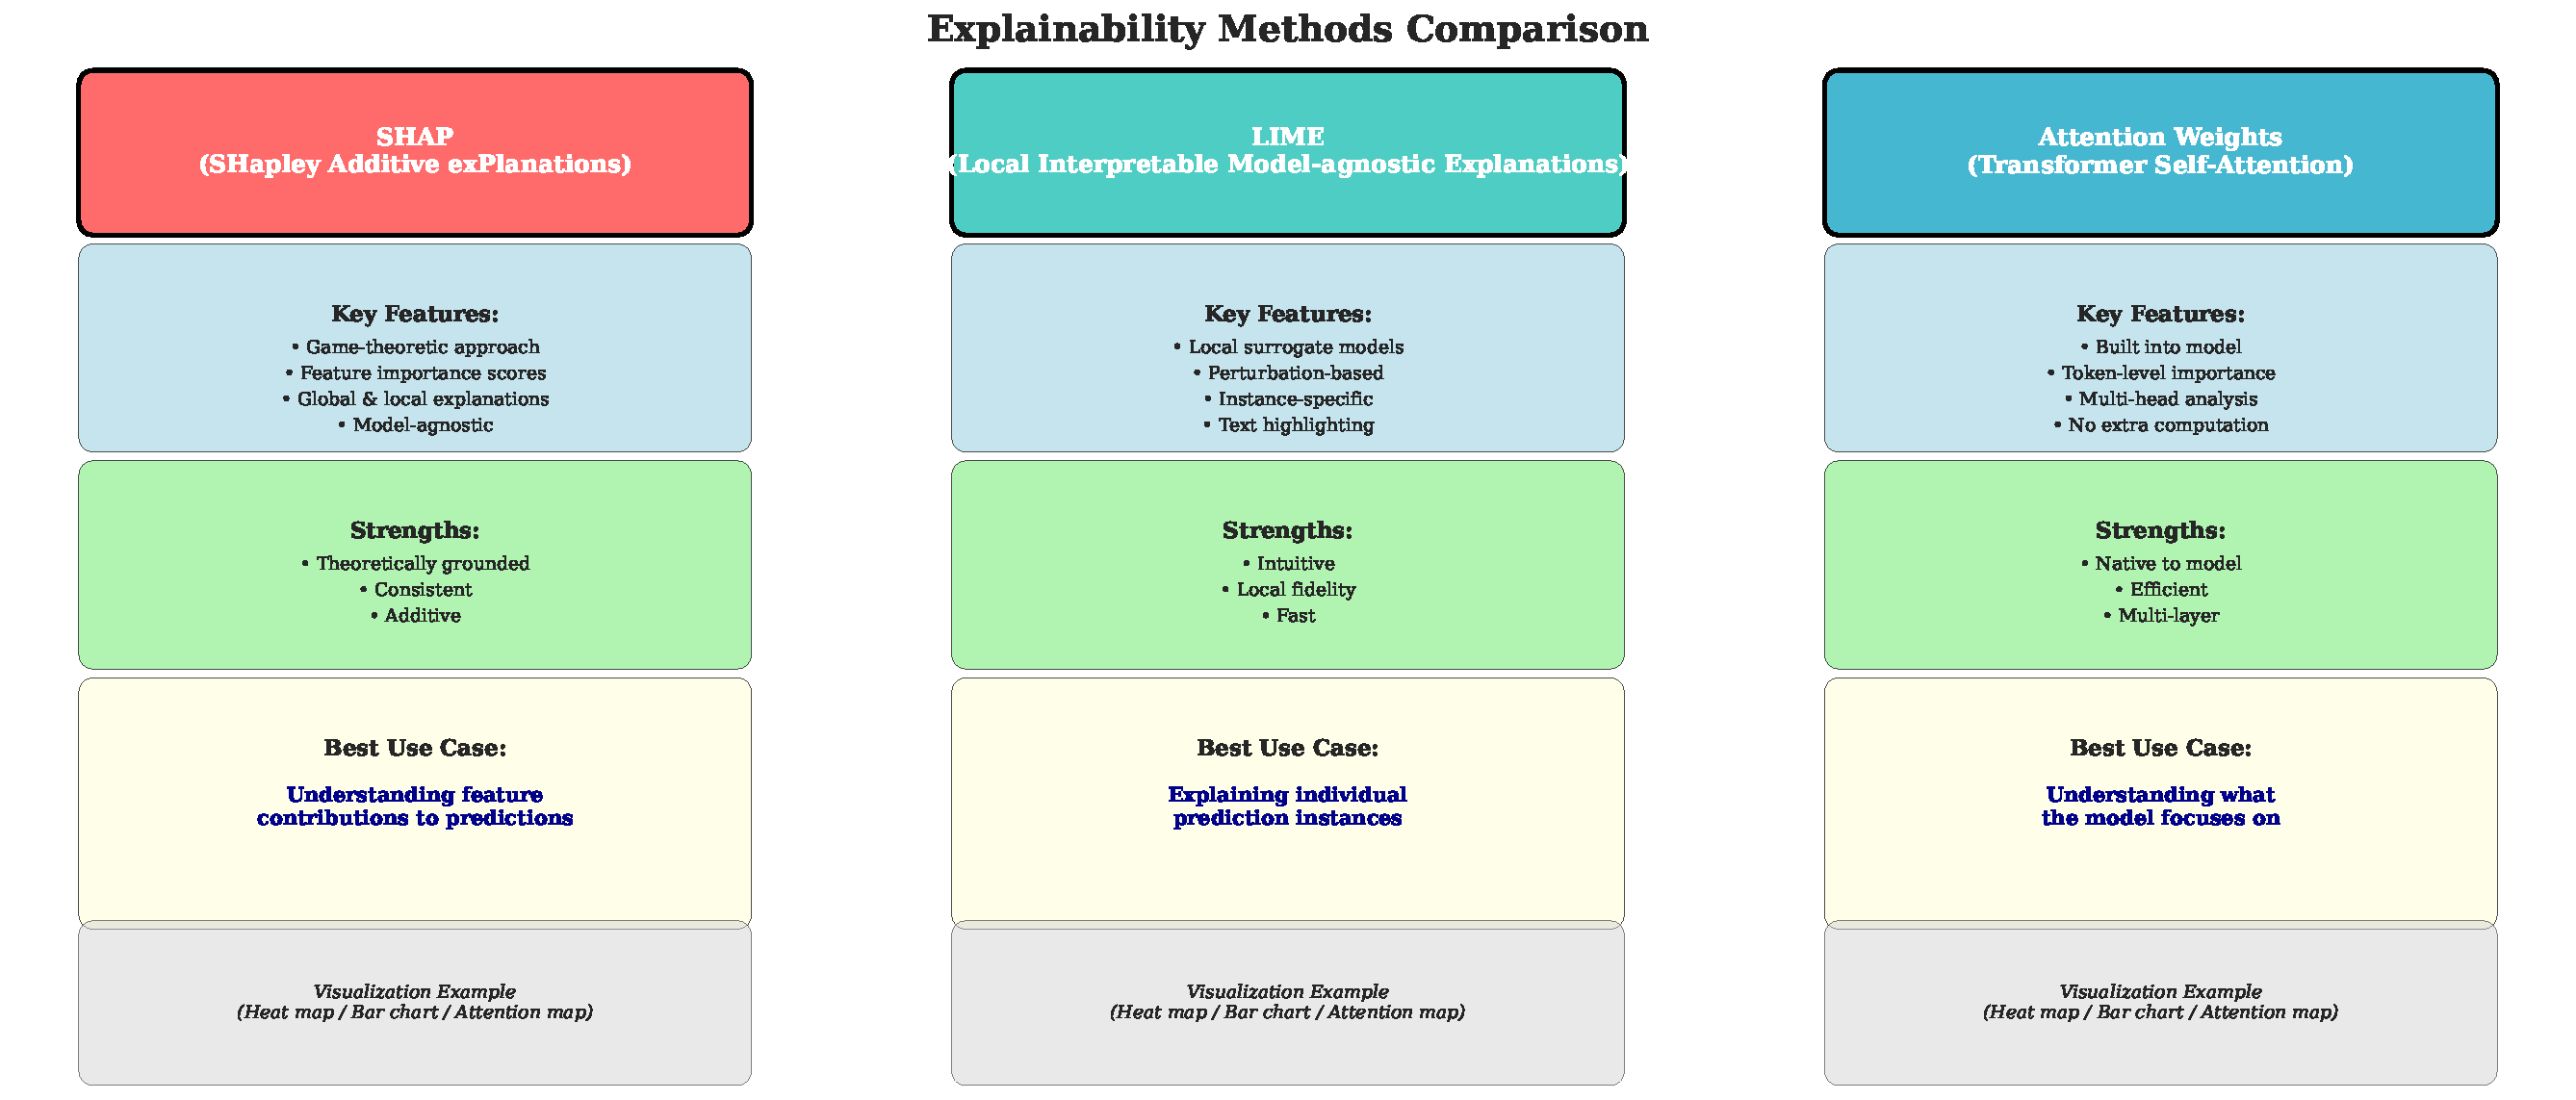
\includegraphics[width=0.95\textwidth]{\figpath/explainability_comparison.pdf}
\end{center}
\end{frame}

\begin{frame}{SHAP Analysis Results}
\begin{columns}
\begin{column}{0.6\textwidth}
\begin{center}
% Include SHAP summary plot
\includegraphics[width=\textwidth]{\figpath/shap_summary_placeholder.png}
\end{center}
\end{column}
\begin{column}{0.4\textwidth}
\textbf{Key Insights:}
\begin{itemize}
    \item \highlight{Legal keywords} have highest importance
    \item \highlight{Contextual terms} provide disambiguation
    \item \highlight{Clause structure} influences predictions
    \item \highlight{Negations} significantly impact scores
\end{itemize}

\vspace{0.5cm}
\textbf{Top Features:}
\begin{enumerate}
    \item "terminate", "termination"
    \item "liable", "liability" 
    \item "confidential", "proprietary"
    \item "payment", "due"
\end{enumerate}
\end{column}
\end{columns}
\end{frame}

\begin{frame}{LIME Local Explanations}
\begin{center}
% Include LIME explanation example
\includegraphics[width=0.9\textwidth]{\figpath/lime_example_placeholder.png}
\end{center}

\textbf{Example Explanation:} Termination clause prediction
\begin{itemize}
    \item \textcolor{red}{Negative words}: "agreement", "contract" (common in all clauses)
    \item \textcolor{green}{Positive words}: "terminate", "30 days notice", "breach"
    \item Local model accuracy: 0.92
\end{itemize}
\end{frame}

\begin{frame}{Attention Weight Analysis}
\begin{columns}
\begin{column}{0.6\textwidth}
\begin{center}
% Include attention heatmap
\includegraphics[width=\textwidth]{\figpath/attention_heatmap_placeholder.png}
\end{center}
\end{column}
\begin{column}{0.4\textwidth}
\textbf{Attention Patterns:}
\begin{itemize}
    \item \highlight{Multi-head attention} focuses on different aspects
    \item \highlight{Legal terms} receive high attention
    \item \highlight{Clause boundaries} show attention peaks
    \item \highlight{Syntactic structure} influences attention flow
\end{itemize}

\vspace{0.5cm}
\textbf{Layer Analysis:}
\begin{itemize}
    \item Early layers: syntactic patterns
    \item Middle layers: semantic concepts
    \item Late layers: task-specific features
\end{itemize}
\end{column}
\end{columns}
\end{frame}

\begin{frame}{Method Comparison \& Consistency}
\begin{table}[h]
\centering
\begin{tabular}{@{}lccc@{}}
\toprule
\textbf{Metric} & \textbf{SHAP} & \textbf{LIME} & \textbf{Attention} \\
\midrule
Consistency Score & 0.84 & 0.79 & 0.72 \\
Faithfulness & 0.91 & 0.88 & 0.76 \\
Stability & 0.87 & 0.82 & 0.69 \\
Computation Time (ms) & 245 & 156 & 12 \\
\bottomrule
\end{tabular}
\end{table}

\vspace{0.5cm}
\textbf{Key Findings:}
\begin{itemize}
    \item \highlight{SHAP} provides most consistent explanations
    \item \highlight{LIME} offers good balance of speed and quality
    \item \highlight{Attention} is fastest but less faithful
    \item All methods show \highlight{reasonable agreement} on important features
\end{itemize}
\end{frame}

\begin{frame}{Explainability Insights for Legal Practice}
\textbf{Practical Applications:}
\begin{itemize}
    \item \highlight{Contract review acceleration} - focus attention on model-identified key terms
    \item \highlight{Quality assurance} - verify model reasoning aligns with legal knowledge
    \item \highlight{Training support} - help junior lawyers understand clause identification
    \item \highlight{Risk assessment} - understand model confidence in different contexts
\end{itemize}

\vspace{0.5cm}
\textbf{Legal Professional Feedback:}
\begin{itemize}
    \item SHAP explanations most trusted by domain experts
    \item LIME provides intuitive instance-specific insights
    \item Attention visualizations help understand model focus
    \item Combined approach preferred for comprehensive analysis
\end{itemize}
\end{frame}
